\documentclass[12pt]{article}

%%%\usepackage{fullpage}
\usepackage{graphicx}
\usepackage{epsfig}
%%%\textwidth=6.00in \textheight=8.75in \hoffset+0.28in
%%%\voffset+0.16in

\renewcommand{\baselinestretch}{1.5}
%%%\renewcommand{\topfraction}{0.98}
%%%\renewcommand{\bottomfraction}{0.5}
%%%\renewcommand{\floatpagefraction}{0.98}
%%%%
\newcommand{\E}{\mbox{\rm E}}
\newcommand{\lik}{\mbox{\rm lik}}
\newcommand{\logit}{\mbox{\rm logit}}
\newcommand{\factor}{\mbox{\rm factor}}
\newcommand{\var}{\mbox{\rm var}}
\newcommand{\SE}{\mbox{\rm SE}}
\newcommand{\vb}[1]{\mbox{\rm v}\!\left(#1\right)}
\newcommand{\vbt}[1]{\mbox{\rm v}_{[t]}\!\left(#1\right)}
\newcommand{\corr}{\mbox{\rm corr}}
\newcommand{\cov}{\mbox{\rm cov}}
\newcommand{\Eb}[1]{\E\!\left(#1\right)}
\newcommand{\varb}[1]{\var\!\left(#1\right)}
\newcommand{\corrb}[1]{\corr\!\left(#1\right)}
\newcommand{\covb}[1]{\cov\!\left(#1\right)}
\newcommand{\TRT}{\mbox{\rm TRT}}
%%%%

\begin{document}
\title{\bf Optimal Two-Stage Phase II Designs with Long-Term Endpoints}
\author{Bo Huang, Enayet Talukder, and Neal Thomas\\
Pfizer, Inc.}
\date{{ September 29th, 2008}}
\maketitle

\begin{center}
{\bf Abstract}
\end{center}

Phase II trials are often designed with an interim analysis so they can be stopped early if a drug
is ineffective. One problem with interim analyses is incomplete follow-up for some patients.
Standard designs such as Simon(1989) require suspension of accrual until patient follow-up is
completed. Case and Morgan (2003) presented a two-stage design for a phase II oncology trial with a
long-term endpoint that does not suspend accrual when the interim analysis is conducted.  We review
the Case and Morgan design and propose modifications to ensure protection of Type I error and
improved robustness to non-optimal conditions likely to be encountered in practice.  Software (R
package) is described to create the optimal designs and easily simulate their properties to check
asymptotic approximations and the robustness of the performance of the designs in operational
conditions.

\newpage

\section{Introduction}
Phase II oncology trials are undertaken to  assess the activity of a new treatment with activity
most frequently defined in terms of tumor response. With some of the new targeted therapies, it may
not be appropriate to use tumor shrinkage to evaluate activity. Instead, the primary endpoint is
time to death, time to progression, or some other endpoints that must be evaluated over a longer
time period.

Phase II trials are often designed with an interim analysis so they can be stopped early if a drug
is ineffective. However, when the primary endpoint requires a longer observation period, interim
analyses are challenging because of incomplete follow-up for some patients at the time of the
interim analysis.  Standard designs such as Simon (1989) require suspension of accrual while
patient follow-up is completed.  Case and Morgan (2003) presented a two-stage design for a phase II
oncology trial with a long-term endpoint that does not suspend accrual while the interim analysis
is conducted.  They proposed to use the Kaplan-Meier or Nelson-Aalen estimators of the event
probability, using methods like those in Lin et al (1996). Estimation at the time of the interim
analysis includes patients with partial follow-up without necessitating trial suspension, as also proposed by Jennison and Turnbull (2000).  The
design minimizes either the expected sample size, expected duration of accrual, or the expected
total study length under the hypothesis that the drug is ineffective. The null hypothesis for the
new design is an (assumed) known event-free rate within a specified time, which has been judged to
represent ineffective treatment.  This is similar to  the hypothesis in the Simon design, but with
much longer specified times for events to occur.  Schaid, Wieand, and Therneau (1990) proposed a
similar design using the log rank statistic, which also incorporates patients with incomplete
follow-up;  the log rank statistic is not evaluated here, but could be inlcuded as a future
software option.


Both Lin et al (1996) and Case and Morgan (2003) assume a constant accrual rate throughout the
trial, which is not typical in practice. We further investigate the design properties by
generalizing the accrual distribution to have different accrual rates in user-specified intervals.
As noted in Case and Morgan (2003), when only partial follow-up data are available, the level of
the testing procedure can depend on the assumed accrual distribution and the assumed time-to-event
distribution under the null hypothesis.  We evaluate an optimal design and corresponding analysis
that ensure the Type I error rate is below the target level.  The reduction in power or
corresponding increase in sample size necessary to achieve the conservative type I error rates is
also evaluated.

The theoretical derivations of the optimal designs specify a fixed time to end the first stage of
accrual and to conduct the interim analysis, with corresponding projected sample size. Case and
Morgan (2003) also evaluated a modified interim timing rule that ends the first stage when the
projected number of patients has been accrued regardless of the planned interim time. They showed
this rule has more robust statistical properties when the accrual rate is mis-specified.  We also
evaluate this interim timing rule and an additional rule based on the projected patient exposure at
the optimal interim time. This rule not only accounts for the number of patients actually accrued,
but also the length of time patients have been observed. All of the interim timing rules can be
easily applied in practice.

An R package was created to generate the optimal designs and resulting analyses. The package
includes code to perform simulations to validate the theoretical calculations, some of which depend
on asymptotic approximations.  The package also has several options for evaluating a proposed
design under conditions that differ from those assumed when the design was created.


In Section \ref{surv}, we summarize the method for estimating the survival function, based on the
properties in Lin et al. (1996), and indicate the change needed for more general accrual
distributions. In Section \ref{excmdes}, we summarize the design of Case and Morgan (2003) with
necessary modifications. The basic design and analysis is further modified to ensure preservation
of Type I error in Section \ref{consdes}. Methods for adjusting the timing of the interim analysis
so that study conditions match the design assumptions are presented in Section \ref{timesect}.
Optimal designs for an example involving colon cancer are evaluated under non-optimal conditions
that are likely to attain in practice in Section \ref{example}. A detailed optimization algorithm
implemented in an R package is presented in Appendix \ref{optsect}.

\section{Statistical Analysis of the Survival Function}

\label{surv}
 Following Lin et al (1996), assume $n$ patients are accrued to a trial at study times $Y_1,\cdots, Y_n$ (min($Y_i$)=0).
Let $T_1,\cdots,T_n$ denote the event times, which are measured from study entry for each patient.
The targeted length of event-free time is denoted by $x$, which is also measured from study entry
for each patient.  It is assumed there is no unplanned loss to follow-up. The $(Y_i,T_i), i=1,\cdots,n$ are
assumed to be independent and identically distributed throughout. The survival function for $T_i$
is denoted by $S$, the hazard function by $h$, and the cumulative hazard function by $\Lambda$.

At study time $t$ we observe for each individual either an event time $T_i$,censoring at
time $x$, or censoring at time $t-Y_i<x$, whichever comes first. That is, we observe the time $X_i(t)=\min(T_i, x, (t-Y_i)_+
)$ and the event indicator $\Delta_i(t)=I\{T_i\leq \min(x, (t-Y_i)_+)\}$, with $(\bullet)_+$
denoting the positive part. Let $\hat S(x;t)=e^{-\hat\Lambda(x;t)}$ denote the estimate of the
event-free rate through study time $x$ evaluated at time $t$ based on the Nelson-Aalen estimator of
the cumulative hazard function:
$$\hat\Lambda (x;t)=\sum_{i=1}^{n} \frac{\Delta_i(t)}{R_i(t)} \hspace{0.2cm} \mbox{with}
\hspace{0.2cm} R_i(t)=\sum_{j=1}^{n} I\{X_j(t)\geq X_i(t)\} \  .$$

The process,
$n^{\frac{1}{2}}\{\hat\Lambda(x;t)-\Lambda(x)\}$, is asymptotically
Gaussian provided $\Pr(t-Y_i>x)>0$.  Assuming no loss to follow-up and independently distributed $Y_i$, the process has
asymptotic variance
\begin{eqnarray}
\sigma^2(x;t)&=&\int_0^x \frac{h(u)}{\Pr(X_i(t)\geq u)}du \nonumber \\
&=& \int_0^x \frac{h(u)}{S(u)\Pr(Y_i\leq t-u)}du \ . \label{vareq}
\end{eqnarray}
The hazard and survival functions under the null and alternative hypotheses are denoted by
$h_0$, $S_0$, and $h_1$, $S_1$, respectively, and the
corresponding variances in (\ref{vareq}) are denoted by $\sigma_0^2(x;t)$ and $\sigma_1^2(x;t)$.
The variance in (\ref{vareq}) contains a general expression for the accrual distribution,
$\Pr(Y_i\leq t-u)$.

Case and Morgan evaluated designs assuming that the accrual distribution is uniform over time, with
the rate of accrual specified as a design input.  The form of $\Pr(Y_i\leq t-u)$ is generalized here so
that accrual is uniform in pre-specified time intervals, with possibly different accrual rates in
each interval. The model is flexible enough to reflect the typically slow accrual during early site
startup, and the potential slowing of recruitment at some sites in the later stages of the trial.
The density of $Y_i$ is constant within pre-specified intervals, with the expected numbers of patients
starting the study in each interval equal to the projected numbers that can be accrued in the
interval.

The pre-specified time intervals are determined by $b$ boundaries denoted by $0<B_1<\ldots<B_b$.  The numbers of patients that can be accrued in the intervals are denoted by $m_1,\ldots,m_b$.
If the maximum number of patients that can be accrued, $\sum_{j=1}^b m_j>n$, then the
final accrual period(s) will be shortened.

    Setting $F_n(t)=\Pr(Y_i\leq t)$:
    $$F_n(t)=\left\{
    \begin{array}{ll}
    \frac{m_1}{n}\frac{t}{B_1}, & 0<t\leq B_1\\
    \frac{m_1}{n}+\frac{m_2}{n}\frac{t-B_1}{B_2-B_1}, & B_1<t\leq B_2\\
    \vdots & \vdots\\
    \frac{\sum_1^{l-1} m_j}{n}+\frac{n-\sum_1^{l-1} m_j}{n}\frac{t-B_{l-1}}{MDA-B_{l-1}}, &
    B_{l-1}<t\leq MDA\\
    1, & t>MDA
    \end{array}\right.$$
with $l$ is chosen so that $\sum_1^{l-1} m_j<n\leq \sum_1^l m_j$, and the MDA (maximum duration of
accrual) is given by
\begin{equation}
MDA=B_{l-1}+(B_l-B_{l-1})\frac{n-\sum_1^{l-1} m_j}{m_l} \ . \label{MDA}
\end{equation}
When $l=1$, $F_n(t)=min\{\frac{t}{MDA},1\}$, $MDA=B_1\frac{n}{m_1}$, the constant
accrual case in Lin et al (1996) and Case and Morgan (2003).


Lin et al (1996) recommend assessing the hypothesis $H_0: S(x)=S_0(x)$ versus the one-sided alternative $H_1: S(x)>S_0(x)$ at study time $t$ using the asymptotically standard normal test statistic
computed from the $\log$ of the cumulative hazard function (i.e., the log of the event-free rate):
\begin{equation}
Z(x;t)=\frac{n^{\frac{1}{2}}\left\{\ln\left(\Lambda_0(x)\right)-\ln\left(\hat\Lambda(x;t)\right)\right\}\hat\Lambda(x;t)}{\left\{\hat\sigma^2(x;t)\right\}^{\frac{1}{2}}} \ ,
\label{Zeq}
\end{equation}
where
\begin{eqnarray}
\hat\sigma^2(x;t)=\sum_{\left\{i: X_i(t)\leq x\right\}}  \frac{\Delta_i(t)}{R_i^2(t)/n}
\ .
\end{eqnarray}
{\bf Comments:}
\begin{itemize}
\item
Case and Morgan (2003) reversed the order of $\ln\left(\Lambda_0(x)\right)$ and
$\ln\left(\hat\Lambda(x;t)\right)$ in the formula for $Z$. The goal is to reduce the number of
events, which is indicated by a positive value of $Z$ (a lower hazard in the treated group).
\item
The standard error is evaluated at the estimated parameter value, analogous to a Wald test. An alternative could be obtained with the standard error computed using the null value, analogous to the
score test, a more robust and powerful test for small sample sizes (Agresti, 2002).
\end{itemize}

The $\hat\sigma^2(x;t)$ estimates the asymptotic variance of $\hat\Lambda(x;t)$ under both the null and
alternative hypotheses, $k=0,1$. The asymptotic standard error of $\sqrt{n}
\big(\ln(\Lambda(x))-$ $\ln(\hat\Lambda(x;t))\big)$ is $\sigma_k(x;t)/\Lambda(x)$, which is estimated by
$\hat\sigma/\hat\Lambda$.  The transformation is applied to improve the asymptotic normal
approximation. Let $I_k(x;t)\equiv 1/\sigma_k^2(x;t)$ denote the information available for
estimating $\Lambda(x)$ at study time $t$, with $k=0,1$ for the null and alternative
distributions. The joint distribution of $Z(x;t)$ and $Z(x;t^*)$ at two study times $t$, $t^*$ is asymptotically
bivariate normal with correlation given by
\begin{equation}
\rho_k(t,t^*)=\sqrt{I_k(x,t)/I_k(x,t^*)} \ , \label{eqnrho}
\end{equation}
where $t\leq t^*$ and $k=0,1$ (Lin et al, 1996).  Note that $\rho_k(t,t^*)$ is also the square root of the ratio of information for estimating $\ln\left(\Lambda(x;t)\right)$ and
$\ln\left(\Lambda(x;t^*)\right)$, because the derivative terms ${\Lambda(x)}^{-1}$ in the asymptotic variances cancel.

It is assumed that there is no loss to follow-up, which may not be true, depending on how
event-free times are defined. We can further define a
censoring variable $V_i$ for patient $i$ and assume the random triplets $(Y_i, T_i, V_i)$ are
independent and identically distributed. The analyses in the section can be generalized, for
example, $\Delta_i(t)=I\{T_i\leq \min(x, V_i, (t-Y_i)_+)\}$. For the purpose of creating designs,
however, we do not account for unplanned loss to follow-up.

\section{The Sequential Design of Case and Morgan (2003)}
\label{excmdes}

Consider a phase II design with a single interim analysis conducted at a pre-specified time.
At the interim analysis, the trial may be stopped for futility (low response or event-free rate),
but it will not be stopped for a positive efficacy outcome.  Accrual is not suspended at the time of the interim analysis.  Following the notation and
derivations in Case and Morgan (2003) with some minor modifications: \vskip 24pt

\noindent $MDA$ : Maximum duration of accrual, which is the time to accrue all patients if the
study does not stop at the interim analysis.

\noindent $MTSL$ : Maximum total study length=$MDA+x$.

\noindent $t_1$ : Time at the interim analysis.

\noindent $t_2$ : Time from the interim analysis to the end of accrual assuming the study does not
stop at the interim analysis.  If the interim analysis occurs after the end of accrual, $t_2$ is $0$.

\noindent $n$ :  The maximum sample size if both stages of the trial are completed.

\noindent $n_1$ : Number of patients accrued at the time of the interim analysis ($t_1$). The $n_1$ can
equal $n$ if the interim analysis occurs after all patients have been accrued but before the
maximum total study length ($MTSL$).

\noindent $n_2$ : Number of patients accrued between the interim analysis ($t_1$) and the end of
accrual. If the interim analysis occurs after the end of accrual, $n_2=0$.

\noindent $P_s$ : Probability of stopping at $t_1$ under $H_0$.

\noindent $EDA$ : Expected duration of accrual = min($t_1$, $MDA$)$+(1-P_s)t_2$, calculated under
$H_0$.  When $t_1>MDA$, $EDA=MDA$.

\noindent $ESS$ : Expected sample size = $n_1+(1-P_s)n_2$, which is calculated under $H_0$.

\noindent $ETSL$ : Expected total study length = $t_1+(1-P_s)(MTSL-t_1)$, which is calculated under
$H_0$.

\noindent $I_{1k}$, $k=0,1$: Information at $t_1$ under the null and alternative hypotheses.

\noindent $I_{max,k}$, $k=0,1$: Information at $MTSL$ under the null and alternative hypotheses.
\vskip12pt

\noindent Note that $MDA$ and $MTSL$ are pre-specified fixed quantities.  The other quantities are
derived from them, the accrual distribution, and the survival functions specified in Section
\ref{surv}.  The two-stage design proceeds as follows. \vskip12pt

\noindent Stage 1: Accrue $n_1$ patients between time $0$ and time $t_1$. Each patient is followed
until they have an event or successfully reach time $x$, or until study time $t_1$, whichever is
first. Calculate the Z-statistic in (\ref{Zeq}), and denote it by $Z_1(x;t_1)$. If
$Z_1(x;t_1)<C_1$, stop the study for futility; otherwise, continue to the next stage. The optimal
time for the interim analysis, $t_1$,  the total number of patients, $n$, and test boundary, $C_1$,
will be derived as part of the design.  The probability of stopping under the null hypothesis is approximated by $P_s=\Phi(C_1)$, where $\Phi$ is the standard normal cummulative distribution function.  The $n_1$ is  a random variable determined by $t_1$ and the accrual
distribution.\vskip12pt

\noindent Stage 2: Accrue $n_2$ additional patients between times $t_1$ and $MDA$. Follow all
patients (both stages) until they have an event or successfully reach time $x$, then calculate a
second $Z$ statistic, denoted by $Z_2(x;MTSL)$, and reject $H_0$ if $Z_2(x;MTSL)>C_2$.  The test
boundary, $C_2$ will also be derived as part of the optimal design. \vskip 24pt


The non-parametric estimator $\hat\Lambda(x;t)$ is defined for any value of $t>x$, so an interim
analysis (i.e., $t_1$) could be done anytime after time $x$  and before time $MTSL$.  If $t_1$ is
close to $x$, the interim analysis will be based on a small effective sample size.  The maximum amount of information
for estimating $\Lambda(x)$ is $I_{max,k}=I_k(x,MTSL)$, which is achieved at any $t\geq MTSL$. The
joint distribution of $Z_1$ and $Z_2$ is bivariate normal with correlation
$\rho_0=\sqrt{I_{10}/I_{max,0}}$ under $H_0$, and $\rho_1=\sqrt{I_{11}/I_{max,1}}$ under $H_1$. The
information at any time $I(x;t)=1/\sigma^2(x;t)$ can be obtained by numerically evaluating equation
(\ref{vareq}).

There are two constraints (Type I and II errors) and four design parameters: $n, t_1, C_1, C_2$. We
assume the accrual distribution throughout the trial is fixed and known. Following Case and Morgan (2003), we obtain solutions that
minimize either the $EDA$, $ESS$ or the $ETSL$ under $H_0$, subject to the constraint that the Type
I error is approximately $\alpha$, and the power is approximately $1-\beta$. Minimizing the $EDA$
and minimizing the $ESS$ are the same in Case and Morgan (2003) as the accrual rate is assumed to
be constant throughout. In the more flexible design setting, however, they may be different, so
minimizing the $ESS$ is more practical. The change required to permit
more general forms of the accrual distribution is that more complex integrals must be evaluated in
the asymptotic variance formula for the estimator in (\ref{vareq}).

From Lin et al (1996), the Type I error is asymptotically approximated by $B(C_1,C_2,\rho_0)$, and
the power is approximated by $B(C_1-\rho_1 u,C_2-u,\rho_1)$, where $B(C_1,C_2,\rho)$ denotes the
bivariate normal probability that $Z_1>C_1$ and $Z_2>C_2$, given a correlation between $Z_1$ and
$Z_2$ of $\rho$, and $u$ is described below.  The $C_1, C_2$ are chosen so that $B(C_1,C_2,\rho_0)=\alpha$
and $B(C_1-\rho_1 u,C_2-u,\rho_1)=1-\beta$.  The $u$ in the power approximation is the mean of $Z_2$
under the alternative hypothesis.  The asymptotic approximations for the Type I error and power are
derived from equations (\ref{vareq}) and  (\ref{Zeq}), and the means of the asymptotic
distributions of $Z_1$ and $Z_2$ under $H_1$ are:

\begin{equation}
\Eb{Z_1\mid
H_1}=\frac{n^{1/2}\left\{\ln\left(\Lambda_0(x)\right)-\ln\left(\Lambda_1(x)\right)\right\}\Lambda_1(x)}{\sigma_{11}}
\ , \label{z1H1}
\end{equation}
\begin{equation}
u\equiv \Eb{Z_2\mid H_1}= \frac{n^{1/2}\left\{\ln\left(\Lambda_0(x)\right)-\ln\left(\Lambda_1(x)\right)\right\}\Lambda_1(x)}{\sigma_{21}} \ , \label{ueq}
\end{equation}
where
\begin{equation}
\sigma_{11}^2\equiv \sigma_{1}^2(x;t_1)=\int_0^{x} \frac{h_1(u)du}{S_1(u)\Pr(Y_i\leq t_1-u)} \ , \label{v11}
\end{equation}
\begin{eqnarray}
\sigma_{21}^2=\sigma_{1}^2(x;MTSL)&=&\int_0^{x} \frac{h_1(u)du}{S_1(u)\Pr(Y_i\leq MTSL-u)} \nonumber\\
 &=& \int_0^{x} \frac{h_1(u)}{S_1(u)}du \  \label{v21}
\end{eqnarray}
Combining equations (\ref{eqnrho}) and (\ref{z1H1}), $\Eb{Z_1\mid H_1}$  becomes $\rho_1 u$.  The
asymptotic variances of $Z_1$ and $Z_2$ equal one by construction under both $H_0$ and $H_1$, with
correlation given by $\rho_0$, $\rho_1$ under $H_0$, $H_1$.

Details of an $R$ algorithm implementing the optimization calculations in this section and a
modified design in the next section are given in Appendix  \ref{optsect}.


\section{A modified analysis and design to preserve Type I error}
\label{consdes}

The two-stage design and resulting analyses are based on evaluation of a non-parametric estimator
of event rates at a single pre-specified time. The correlations between test statistics at the
interim and second stages, $Z_1$ and $Z_2$, which are required for computation of the test
boundaries, $C_1$ and $C_2$, depend on the entire survival curve up to the specified evaluation
time $x$ under both $H_0$ and $H_1$.  These distributions must be specified as a design input;  an
R package {\it OptimPhase2} currently implements Weibull distributions with user-specified
parameters. The dependence of $C_1$ and $C_2$ on the specified distributions is weak, but it does
result in
 dependence of the Type I error and power on the choice of the parametric distributions (see
Case and Morgan (2003) for simulation results).  This dependence can be easily overlooked because
the test statistic is based on non-parametric estimation evaluated at a single event time ($x$).

The dependence of the Type I error rate on the accrual and survival distributions arises because a
small percentage of potential Type I errors during the second stage of testing are avoided when the
trial is terminated at the end of the first stage.  The percentage of potential Type I errors
avoided is typically small because the trial is terminated after the first stage only when the
response (or event-free) rate is low.  Data sequences that yield low first-stage estimates,
followed by high second-stage estimates are rare, with the frequency determined by the correlation
between the estimators at the first and second stages.  The  method described in Section
\ref{excmdes} uses the correlation derived from the accrual and survival distributions to recover
the alpha from the potential Type I errors avoided at the first stage.

The dependence of the Type I error rate on the assumed distributions can be eliminated by including
the Type I errors avoided in the first stage in the calculation of the error rate.  A more
conservative alternative method becomes: choose $C_1, C_2$ so that $\Phi(C_2)=\alpha$ and
$B(C_1-\rho_1 u,C_2-u,\rho_1)=1-\beta$.  This procedure is consistent with regulatory guidance to protect Type I error even with interim analyses where the stated intention is to stop only for futility (FDA, Section 4.3.2, 2006).

Also note that the test based on the normal approximation
at the end of the second stage can be replaced by an exact binomial test (assuming no loss to
follow-up), with the role of the normal approximation reduced to futility testing at the first
stage, and the selection of sample size and timing of the first-stage analysis.

\section{Adjusting the timing of the interim analysis to match observed study conditions}
\label{timesect}

The optimal time to perform the interim analysis, $t_1$, is dependent on correct specification of
the patient accrual and survival distribution.  Case and Morgan (2003) evaluated a modified rule
for the time of the interim analysis based on matching the number of patients actually accrued in
the study to the expected number of patients to be accrued at the time of the interim analysis
under the original design assumptions.  This timing rule for the interim analysis performed better
in their simulations, so it will be evaluated in Section \ref{simulations}.

Further refinement of the timing rule is also possible by matching the observed patient exposure
time to the expected exposure time under the optimal design conditions.  This refinement accounts
for the time patients have been in the study, which is potentially important if many patients are
accrued shortly before the interim analysis, and thus contribute little information to the
estimated event rate at time $x$.

The total expected patient exposure truncated by $x$ under the optimal design assumptions is
\begin{displaymath}
n\E\left(\min\left(x,\left[t_1-Y_i\right]_+\right)\right)=n*\Pr(Y_i\leq t_1)\E\left(\min\left(x,\left[t_1-Y_i\right]_+\right)\mid Y_i\leq t_1\right)
 \ .
\end{displaymath}
The $\Pr(Y_i\leq t_1)$ is evaluated directly from the accrual distribution.  The distribution of $Y_i$ given $Y_i\leq t_1$ is required to compute the conditional expectation.  Find $k$ so
$B_{k-1}<\min(MDA,t_1)\leq B_k$ and truncate this interval at $\min(MDA,t_1)$ so $B_k$ is re-assigned the value $\min(MDA,t_1)$.  The expected accrual, $m_k$, is also re-defined to
$m_k(\min(MDA,t_1)-B_{k-1})/(B_k-B_{k-1})$.  The  proportion and density in each interval of the conditional accrual distribution become $P_j=m_j/\sum_{l=1}^k m_l$ and $D_j=P_j/(B_j-B_{j-1})$,
$j=1,\cdots,k$.

The truncated conditional expected exposure time is then found by summing over the intervals with constant density, which have one of three possible configurations:

\begin{enumerate}
\item
The $t_1-x\geq B_j$, which contributes $x\Pr(Y_i\in (B_{j-1},B_j))=xD_j(B_j-B_{j-1})$.
\item
The $B_j>t_1-x\geq B_{j-1}$, which contributes
\begin{eqnarray*}
&&x\Pr(Y_i\in (B_{j-1},t_1-x))+D_j\int_{t_1-x}^{B_j}(t_1-y)dy = \\
&&xD_j(t_1-x-B_{j-1}) + D_j t_1(B_j-t_1+x) + D_j(B_j^2-(t_1-x)^2)/2 \ .
\end{eqnarray*}
\item
The $t_1-x<B_{j-1}$, which contributes
\begin{displaymath}
D_j\int_{B_{j-1}}^{B_j}(t_1-y)dy=D_jt_1(B_j-B_{j-1})-D_j(B_j^2-B_{j-1}^2)/2 \ .
\end{displaymath}
\end{enumerate}

The number of patients accrued and their truncated exposure are not known at future times, but they
can be reliably projected based on currently accrued patients, and projections of future accrual
for short durations of time (e.g., 2 months), thus permitting practical operational planning for
the interim analysis.  Because exact targeting for accrual and exposure times will not be achieved
in real practice, simulation studies will be included in Section \ref{simulations} to evaluate the
impact of small differences between planned and actual timing of the interim analysis.

Patient exposure is evaluated because we anticipate it will be a better predictor of expected
information than the number of accrued patients.  Exploratory simulations were also performed with
timing rules based on the observed information.  Matching on the observed information did not
improve performance, however, because it depends on the estimated time-to-event distribution, which
is not stably estimated during early accrual.  The observed information was not always a monotone
function of time, and would be difficult to project with sufficient lead time for operational
purposes. Because it did not improve theoretical performance of the designs and analyses, and it
would be hard to implement and explain, the interim timing rule based on the observed information
was not pursued.
\section{Example}
\label{example}

\subsection{Background}

Potential designs based on a recent study involving refractory metastatic adenocarcinoma of the
colon are evaluated to demonstrate the methods that have been implemented to create an optimal
design. We also evaluate the optimal designs under non-optimal conditions.  All of the methods are
implemented by functions in the R package {\it OptimPhase2}.  The primary objective of the study
was to evaluate overall survival at $6$ months from enrollment. The null survival rate at $6$
months was $0.45$ based on the findings of Jonker (2007), Rao, et al (2004), and Van Cutsem, et al
(2007). An alternative rate of $0.60$ or greater was selected as a success rate warranting further
development.  We assume an exponential survival curve for both hypotheses during the design stage,
but the resulting designs are also evaluated by
simulations assuming an accelerating hazard function. It is assumed that $3$ patients can be accrued per month for up to $3.5$ years if
needed for a maximum of $126$ patients.

\subsection{Optimal designs}

Designs were created with targeted one-sided Type I errors of 0.05 or 0.10, and power of 0.80.  The
sample sizes for simple non-sequential designs based on the  normal approximation are $80$  with
$\alpha=0.05$, and $58$ with $\alpha=0.10$.  The corresponding duration of accrual ($DA$) and study
length ($SL$) for the fixed designs are 26.67, 32.67, and 19.33, 25.33 (months).

Two-stage designs were created that recover the $\alpha$ from early stopping, and more conservative
designs that do not recover the $\alpha$ were also created (see Section \ref{consdes}).  The
designs minimize the expected sample size ($ESS$), but the other criteria ($EDA$ and $ETSL$) are
also monitored. The assessment of each optimality criteria is displayed in Figure \ref{optplot} as
a function of potential maximum sample size $n$ for the design with alpha level of $0.05$ and  no recovery of $\alpha$.  The criteria and the
maximum sample sizes are expressed as ratios relative to the values of the single-stage fixed
design with the same Type I error and power.  The $ESS$ and $EDA$ criteria coincide because the
accrual rate is assumed constant.  The $ETSL$ is minimized by a trial with a larger maximum sample
size, but the $ETSL$ curve is nearly flat over a range of designs that includes its optimal sample
size and the optimal size for the $ESS$ criteria. The design is thus robust to the choice of
optimality criteria.  In some settings, a compromise design yielding good but non-optimal results
for all of the criteria can be selected using a plot like Figure \ref{optplot}.  The R-package can
produce two-stage designs for a pre-specified value of the maximum sample size $n$ to support the
choice of compromise designs.

The properties of the two-stage design are sumamrized in Table
\ref{optchar}.  The two-stage designs reduce the expected number of patients by approximately $20$ and the expected
study length by $10$ months when $\alpha=0.05$, and by $8$ patients and $5$ months when
$\alpha=0.10$.  The more conservative combination of design and decision criteria that does not
recover $\alpha$ from the interim analysis requires $2-3$ more expected patients to maintain the same power compared to designs with
$\alpha$ recovery.  The magnitude of the potential saving is dependent on the accrual rate as
little saving is possible if most of the patients are accrued by the time a sufficient number of
patients have reached the time of the endpoint evaluation.  The more information required for the
final decision criteria (i.e., lower $\alpha$, higher $\beta$), the more patients that must be
accrued, and thus  potential reductions from two-stage designs are larger.



\begin{table}[h]
\caption{Optimal Design Characteristics}
\label{optchar}
 \begin{center}
 \begin{tabular}{c|cc|cc}\hline\hline
\vspace{-8pt}&\multicolumn{2}{c}{$\alpha=0.05$}\vrule&\multicolumn{2}{c}{$\alpha=0.10$}\\
&R=Y&R=N&R=Y&R=N\\
\hline
max N& 93&94&65&64\\
interim Time&13.53&14.05&11.18&11.75\\
interim N&41&43&34&36\\
ESS&58.87&61.50&48.16&50.29\\
EDA&19.62&20.50&16.06&16.76\\
ETSL&21.71&22.74&18.84&19.90\\
MTSL&37&37.33&27.67&27.33\\
interim P&0.506&0.495&0.464&0.442\\
final P&0.533&0.538&0.527&0.533\\
\hline \hline\hline \multicolumn{5}{l}{Note:  R=Y,N for recovery of $\alpha$ equal yes/no.}
\end{tabular}
\end{center}
\end{table}

Simulated data were created under conditions matching the design assumptions (e.g., accrual rate,
shape of survival curves).  The results are summarized in Table \ref{optcond}.  Each simulation
setting was replicated $10,000$ times.  The simulation standard errors for estimated proportions
(e.g. $\alpha$ levels) are $\leq 0.003$. The timing of the interim analysis was based on the rules
that match the sample size and the patient exposure under the design assumptions.  Because the
results from the two rules were very close under the design assumptions, the small differences were
averaged for reporting in Table \ref{optcond}.

All of the design and decision criteria produced conservative control of the Type I error when the
target $\alpha=0.05$;  the exact and normal approximation yielded the same rejection rates, but
both differed from the target levels.  The testing procedure based on the normal approximation with
recovery of $\alpha$, however, had Type I error that appreciably exceeded the targeted $0.10$
level.  This is due to the normal approximation errors with interim and final sample sizes of $34$
and $65$.  Approximation errors of this magnitude are common in designs of this size.  Because the
method with $\alpha$ recovery does not sufficiently control the Type I error in some settings, it
is not evaluated in the next section.


All of the designs had power exceeding the targeted $80\%$ level by $1-6$ percent.  The higher
achieved power levels are also due to normal approximation errors.  A tendency to produce higher
than targeted power levels was also noted when the same methods were applied to single-stage fixed
designs with null event-free rates of $40$ percent or higher.  For lower null event-free rates, the
normal approximation tends to produce lower powers than the targeted levels. Corresponding to the
higher power, the expected number of patients was $1-2$ larger than projected for the design under
the null hypothesis, and the expected study length is longer by approximately $0.5$ months.  The
higher powers and larger expected sample sizes occur in part because the frequency of futility
stopping at the interim analysis is slightly lower than projected for the design.  Case and Morgan
(2003) suggested a sample size adjustment based on the ratio of the sample sizes for the fixed
single-stage design from an exact test versus the normal approximation test.  These adjustments
reduce the sample sizes to better approximate the power under ideal conditions in the current
example. Because power tends to be reduced somewhat in more realistic operational conditions, as
evaluated in the next section, the conservative tendency of the designs in the ideal conditions may
be desirable in practice.



\begin{table}[h]
\caption{Simulation results under the optimal design conditions}
\label{optcond}
 \begin{center}
 \begin{tabular}{c|ccc|ccc}\hline\hline
&\multicolumn{3}{c}{Target $\alpha=0.05$}\vrule&\multicolumn{3}{c}{Target $\alpha=0.10$}\\
\hline
\vspace{-8pt}&\multicolumn{1}{c}{Exact}&\multicolumn{1}{c}{Normal}&\multicolumn{1}{c}{Normal}\vrule&\multicolumn{1}{c}{Exact}&\multicolumn{1}{c}{Normal}&\multicolumn{1}{c}{Normal}\\
&\multicolumn{1}{c}{R=N}&\multicolumn{1}{c}{R=N}&\multicolumn{1}{c}{R=Y}\vrule&\multicolumn{1}{c}{R=N}&{R=N}&\multicolumn{1}{c}{R=Y}\\
\hline
$\alpha$&0.040&0.040&0.045&0.070&0.106&0.131\\
Power   &0.842&0.842&0.842&0.816&0.865&0.859\\
ESS     &63.36&63.36&60.05&51.37&51.37&49.35\\
EDA     &20.83&20.83&19.73&16.83&16.83&16.14\\
ETSL    &23.46&23.46&22.16&20.31&20.31&19.31\\
\hline\hline \multicolumn{7}{l}{Note:  R=Y,N for recovery of $\alpha$ equal yes/no.}
\end{tabular}
\end{center}
\end{table}


\begin{figure}[h]
\caption{The optimality criteria displayed for a range of maximum sample sizes.  The criteria and
the maximum sample sizes are expressed as ratios relative to the corresponding value in a
single-stage fixed design ($\alpha=0.05$ is not recovered). } \label{optplot}
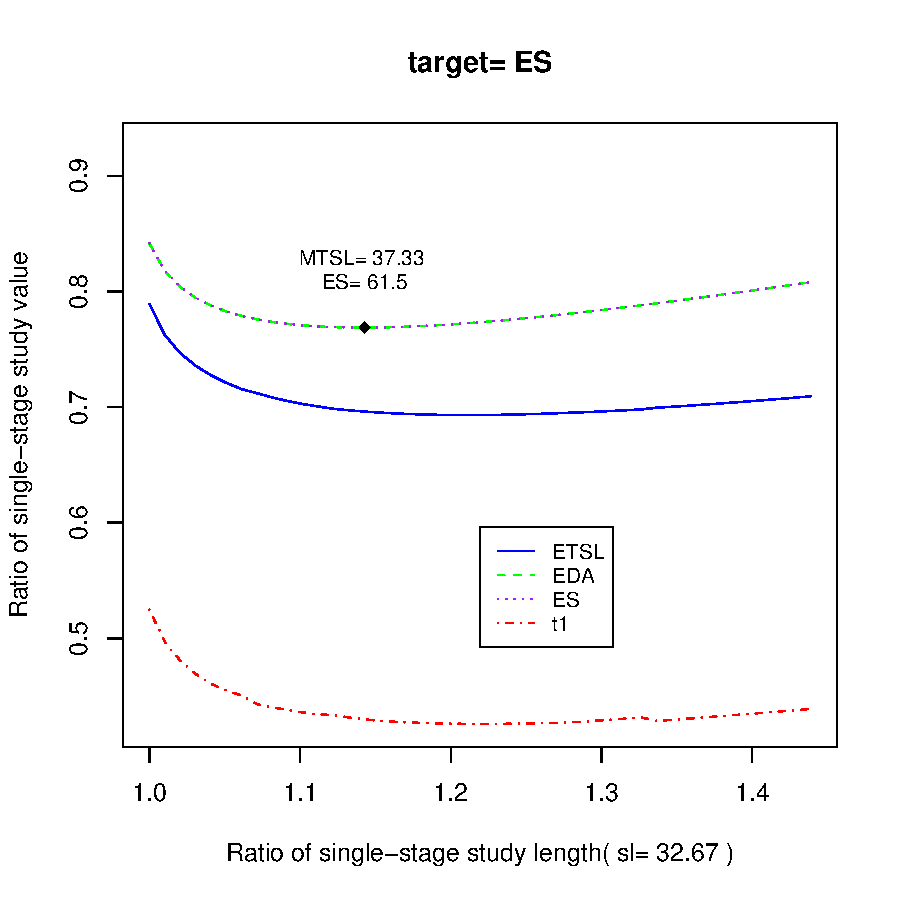
\includegraphics[height=3.85in,width=5in]{design.pdf}
\end{figure}

\clearpage

\subsection{Evaluating optimal designs under non-optimal conditions}
\label{simulations}

Simulations were conducted under several plausible operating conditions that differ from those
assumed when creating the design.  Both of the interim timing methods were evaluated for each simulation setting.  The designs for both levels of
$\alpha$ were evaluated, and reported separately due to differences in performance.

Two sets of survival curves were simulated: 1) the null and alternative exponential curves assumed in the designs, and 2) Weibull distributions with shape parameter of $3$, which yield very few early events and rapidly accelerating hazard close to the endpoint time of $6$ months.  All of the survival curves match the hypothesized values at $6$ months.

The time of the interim analysis was varied from the optimal time to represent operational
constraints. The proportions of the optimal target (sample size or patient exposure) were $1.0$,
$0.95$, and $1.05$.

Three accrual patterns were simulated:  target rate (3 per month), slow starting ($1$ per month for 4 months followed by $3$ per month), and fast accruing ($5$ per month).

The simulation results are summarized in Table \ref{noptcond}.  The Type I errors based on the
exact tests remained conservative and the normal approximation performed adequately, but there were
small elevations of the Type I errors for some settings using the normal approximation.  The power
varied somewhat across the simulation settings, but severe loss in power did not occur.  Matching
on patient exposure reduced the small loss of power in some non-optimal settings compared to
matching on the targeted sample size for the timing of the interim analysis.  These improvements in
power were accomplished by increasing the sample sizes at the interim analyses in some settings
that resulted in small increases in the ESS.

Analysis of variance (ANOVA) was applied to the power and ESS results across the factors in the
simulation to determine the predominant sources of variation.  For power, the dominant factors were the
accrual rate, shape of the survival curve, the accuracy of the timing of the interim analysis, the
method used to time the interim analysis, and the interaction between the interim method and the
accrual rate.  The factors were the same for both $\alpha$ levels.  The lowest power levels
occurred with the fastest accrual, accelerating hazard rate, and smaller than planned interim
sample sample size.  ANOVA applied to the ESS results yielded the same factors except that the
hazard function determining event rates was not predictive.

\begin{table}[h]
\caption{Simulation results under non-optimal conditions}
\label{noptcond}
 \begin{center}
 \begin{tabular}{c|cc|cc}\hline\hline
\vspace{-8pt}&\multicolumn{2}{c}{Target $\alpha=0.05$}\vrule&
\multicolumn{2}{c}{Target $\alpha=0.10$}\\
&E1&N1&E1&N1\\
\hline
$\alpha$ (exact)&0.040&0.039&0.069&0.068\\
&0.039, 0.042&0.036, 0.042&0.066, 0.071&0.063, 0.071\\
\hline
$\alpha$ (normal)&0.040&0.039&0.105&0.103\\
&0.039, 0.042&0.036, 0.042&0.100, 0.109&0.094, 0.108\\
\hline
Power (exact)&0.840&0.828&0.812&0.802\\
&0.807, 0.859&0.769, 0.857&0.784, 0.824&0.762, 0.822\\
\hline
Power (normal)&0.840&0.828&0.860&0.849\\
&0.807, 0.859&0.769, 0.857&0.830, 0.873&0.805, 0.873\\
\hline
ESS&65.80&64.82&52.93&52.31\\
&63.12, 69.72&63.18, 66.76& 50.97, 55.79&51.44, 53.44\\
\hline\hline
\multicolumn{5}{l}{\vspace{-8pt}Note:  E1=matching optimal exposure, N1=matching optimal $n_1$.}\\
\multicolumn{5}{l}{       \vspace{-8pt}The upper number in each cell is the mean across simulation conditions.}\\
\multicolumn{5}{l}{       The lower numbers are the minimum, maximum.}
\end{tabular}
\end{center}
\end{table}

\clearpage


\section{Discussion}

The Case and Morgan generalization of the Simon two-stage design was reviewed and additional
modifications were proposed and evaluated to ensure protection of the Type I error and more robust
performance under likely operational conditions. In settings with slow accrual, long-term endpoint
(e.g. 1-year survival) and a low probability of efficacy, the two-stage designs can reduce the
number of patients exposed to ineffective drugs and reduce time to decisions while maintaining
control of type I error and type II error.

The designs here focused on assessment of the event-free rate at a single time point. Tests based
on such endpoints may be more appropriate than widely used non-parametric rank-based tests (e.g.,
log-rank test) for some regimens and cancer modalities such as immuno-oncology, in which it takes
time for immune activation and building of an immune response, so comparisons to a results from a
regimen yielding faster response might be misleading.  In settings where comparison of
time-to-event curves is more appropriate, the methods described here can be modified to use other
test statistics.  The methods could also be generalized to allow comparison to a concurrently
randomized control group (see for example, Schaid, Wieand, and Therneau, 1990).

Software (R package {\it OptimPhase2}) is available to create optimal designs and explore
alternative compromised designs under different settings. Code to easily generate simulations to
check the asymptotic approximations and performance under non-optimal conditions is also supplied.
A test function is also available to compute the test statistics during the trial conduct.

In addition to the R package, there are other available software sources to generate the original
Case and Morgan's design. For example, the national cancer center in Singapore developed an Early
Phase Clinical Trial (EPCT) software to create some commonly used phase I and phase II cancer
clinical trial designs, including Case and Morgan's. An update version of the EPCT software has
been incorporated into a book (Machin et al, 2008).


\appendix

\section{Optimization Algorithm}
\label{optsect}

An algorithm is specified to minimize either $EDA$, $ESS$ or $ETSL$ is described in Steps 1-11.
The user inputs are:
\begin{description}
    \item[a.]
 The Type I error and power, $\alpha$, $\beta$.
    \item[b.]
    The time to event distributions $S_0$ and $S_1$.  The  method is
implemented with Weibull distributions for $S_0$ and $S_1$, so the user inputs  two parameters per distribution.
    \item[c.]
    The target time to evaluate the survival function, $x$.
    \item[d.]
    The projected accrual during different time periods.  The user
 specifies a set of intervals given by times $0 (\equiv
B_0),B_1,\cdots,B_b$ in which the accrual rates are approximately
constant. The $B_b$ is the longest feasible time to accrue the trial.
The value of $b$ can be one, corresponding to uniformly distributed
accrual throughout the study.  This is the accrual model specified by
Case and Morgan.  Associated with each time interval, $(B_{j-1},B_j)$,
the user inputs the number of patients, $m_j$, that could be accrued within the interval.

  If the Type I error and power constraints cannot be achieved with
the specified accrual, the optimization algorithm will stop and report the problem.
\end{description}
\vskip 24pt

The $11$ steps of the optimization method are:
\begin{enumerate}
    \item
Fix  values for $n$ and $\rho_1$.  Combined with the Type I error and power constraints, these determine all of the remaining parameters as described by steps 2-10.
    \item
Compute the $MDA$ from equation (\ref{MDA}) and form the study entry-time distribution to match the
projected accrual rates input by the user.
    \item
Calculate $\sigma_{21}$ ($H_1$) from equation (\ref{v21}), and similarly for $\sigma_{20}$ ($H_0$) by
replacing $h_1$ and $S_1$ by $h_0$ and $S_0$ in equation (\ref{v21}).
    \item
Obtain $\sigma_{11}$ from $\rho_1=\sigma_{21}/\sigma_{11}$, which
implies $\sigma_{11}=\rho_1\sigma_{21}$.
    \item
Obtain $t_1$ by solving equation (\ref{v11}) for the value of $\sigma_{11}$  computed in the previous step. An unique root exists because
$\sigma_{11}$ is monotone in $t_1$.
    \item
Calculate $t_2=max(MDA-t_1, 0)$.
    \item
Calculate $\sigma_{10}$ from equation (\ref{v11}) by replacing $h_1$ and $S_1$ by $h_0$ and
$S_0$.
    \item
Calculate $\rho_0=\sigma_{20}/\sigma_{10}$.
    \item
Calculate $u$ from equation (\ref{ueq}).
    \item
Obtain $C_1$ and $C_2$.
When recovery of $\alpha$ is specified (Section \ref{excmdes}), solve:
$$\left\{\begin{array}{ll} B(C_1,C_2,\rho_0)-\alpha=0 & (A)\\ B(C_1-\rho_1
u,C_2-u,\rho_1)-(1-\beta)=0 & (B)
\end{array}\right.$$
The two-variable equations are solved using R function {\it optim}(). The idea is to minimize
$(A)^2+(B)^2$ to 0 (if possible, otherwise no solution), and the minimizers $\hat C_1$ and $\hat
C_2$ are the desired roots. The default setting is to minimize $(A)^2+(B)^2$ to within $1e^{-6}$.
When recovery of $\alpha$ is not specified (Section \ref{consdes}), solve:
$$\left\{\begin{array}{ll} \Phi(C_2)-\alpha=0 & (A)\\ B(C_1-\rho_1
u,C_2-u,\rho_1)-(1-\beta)=0 & (B)
\end{array}\right.$$
$C_2$ can be computed using the inverse normal CDF supplied in R.  The remaining equation is
monotone in  $C_1$, and is solved for $C_1$ using the $uniroot$ function.
    \item
The optimal design to minimize the $EDA$, $ESS$ or $ETSL$ is found by evaluating all possible $n$.
The optimal $\rho_1$ for each $n$ is found using a combination golden-section search and parabolic
interpolation minimization as described by Brent (1973). It is implemented by the function {\it
optimize}() in R {\it stats} package. The range of $\rho_1$ is between 0 and 1. The search for
optimal $n$ can begin with the fixed sample size of the single-stage design. The two-stage design
requires a larger maximum sample size than a single stage design with the same $\alpha$ and
$\beta$. and thus, the fixed sample size is a lower bound. The fixed sample size $n_0$ for a
1-sided test with a normal approximation is
\begin{displaymath}
n_0=\left[\frac{\sigma_{21}(Z_\alpha+Z_\beta)}{\left\{\ln\left(\Lambda_0(x)\right)-\ln\left(\Lambda_1(x)\right)\right\}\Lambda_1(x)}
\right]^2 \ .
\end{displaymath}
\end{enumerate}
The upper limit for $n$ is input by the user, which is $\sum_1^b m_j$.

\begin{thebibliography}{}
\bibitem{agresti02} Agresti, A. (2002). Categorical Data Analysis. {\it New York: Wiley}
\bibitem{brent73} Brent, R. (1973). Algorithms for minimization without derivatives. {\it Englewood Cliffs: Prentice Hall}
\bibitem{cm2003} Case L.D. and Morgan, T.M. (2003). Design of phase II cancer trials evaluating survival probabilities. {\it BMC Medical Research Methodology} {\bf 3}: 6
\bibitem{guide06} Food and Drug Administration (2006).  Guidance for Clinical Trial Sponsors:  Establishment and operation of clinical trial data monitoring committees.  {\it OMB Control No. 0910-0581}
\bibitem{Jen2000} Jennison, C, and Turnbull, B (2000).  Group Sequential Designs with Applications to Clinical Trials.  {\it Boca Raton: Chapman Hall/CRC}
\bibitem{jonker07} Jonker DJ et al. (2007).  Abstract No. LB-1, {\it American Association for Cancer Research}
\bibitem{km58} Kaplan, E.L. and Meier, P. (1958). Nonparametric estimation from incomplete observations. {\it Journal of American Statistical Association}. {\bf 53}: 457-481
\bibitem{lin96} Lin, D.Y., Shen, L., Ying, Z. and Breslow, N.E. (1996). Group sequential designs for monitoring survival probabilities. {\it Biometrics}. {\bf 52}: 1033-1042
\bibitem{machin08} Machin, D., Campbell, M., Tan, S.B. and Tan, S.H. (2008). Sample Size Tables for
Clinical Studies. {\it Blackwell}
\bibitem{nelson69} Nelson, W. (1969). Hazard plotting for incomplete failure data. {\it J Quality Technology}. {\bf 1}: 27-52
\bibitem{rao04} Rao S, Cunningham D, de Gramont A, et al (2004).  Phase III double-blind placebo-controlled study of farnesyl transferase
inhibitor R115777 in patients with refractory advanced colorectal cancer.
{\bf 22(19)}: 3950-3957
\bibitem{schaid90} Schaid, D., Wieand, S., and Therneau, T. (1990).  Optimal two-stage screening designs for survival comparisons. {\it Biometrika}.
{\bf 77}: 507-513
\bibitem{simon89} Simon, R. (1989). Optimal two-stage designs for phase II clinical trials. {\it Controlled Clinical Trials}. {\bf 10}: 1-10
\bibitem{vc07} Van Cutsem E, Peeters M, et.al. (2007).  Open-label phase III trial of panitumumab plus best
supportive care compared with best supportive care alone in patients with
chemotherapy-refractory metastatic colorectal cancer. {\it Journal of Clinical Oncology}. {\bf 1;25(13)}:1658-1664.
\end{thebibliography}


\end{document}
